\documentclass{beamer}

% Theme choice (you can change to Madrid, CambridgeUS, etc.)
\usetheme{Madrid}

% Optional packages
\usepackage[utf8]{inputenc}
\usepackage{graphicx} % for including images
\usepackage{amsmath, amssymb} % for math symbols
\usepackage{hyperref} % for clickable links
\usepackage{tikz}

% Title info
\title[Short Title]{Factor Models of Returns}
\author[Your Name]{Oden Petersen}
\date{\today}

% Section headers
\AtBeginSection[]{
	\begin{frame}
	\vfill
	\centering
	\begin{beamercolorbox}[sep=8pt,center,shadow=True,rounded=True]{title}
		\usebeamerfont{title}\insertsectionhead\par%
	\end{beamercolorbox}
	\vfill
	\end{frame}
}

\begin{document}

% Title page
\begin{frame}
	\titlepage
	\begin{center}
		\textit{``$y=X\beta+\epsilon$, the rest is commentary.''}
	\end{center}
\end{frame}

\begin{frame}{About Me}
\end{frame}

% Table of contents
\begin{frame}{Outline}
	\tableofcontents
	%% Good to include concrete data examples throughout
\end{frame}

% Section 1
\section{Securities Markets}

\begin{frame}{Spot Transactions}
	The point of trading is to obtain an asset by giving up money, or obtain money by giving up an asset.

	If I give you $q$ units of some asset $A$, and you give me $\$p$, then:
	\begin{itemize}
		\item I have \textbf{sold} $q$ units of $A$ to you at $\frac{\$p}{q}$
		\item You have \textbf{bought} $q$ units of $A$ from me for $\frac{\$p}{q}$
	\end{itemize}

	Buying and selling are collectively called `trading'.

	Suppose I own some amount of $A$ and some amount of money. If we let $s$ be $+1$ for buying and $-1$ for selling, then the result of any trade is to add $qs$ to the amount of $A$ I own, and add $-qps$ to the amount of money I have. %s is called the sign of the trade

	% Stock image of retail store
\end{frame}

\begin{frame}{Securities Markets and Exchanges}
	The \textbf{\textcolor{blue}{market}} is the collective activity of all traders. When we don't care who we trade with, we can just `trade with the market'.

	A \textbf{\textcolor{red}{securities} \textcolor{blue}{market}} for some asset $A$, open at a time $t$, is any \textcolor{red}{standardised} \textcolor{blue}{way for traders to reach agreements to buy or sell} $A$ at a specified \textbf{settlement time} $T\geq t$. %"securities" because of standardisation and regulation

	\pause

	For example, $T=\ldots$
	\begin{itemize}
		\item $t$ (`spot', e.g. blockchain) %ASX tried to do blockchain, this was scrapped in 2022 after 7yrs
		\item $t+1, t+2, \ldots$ (`clearing', e.g. equities)
		\item Last Thursday of month (`futures')
	\end{itemize}

	\pause
	If you agree to give something to someone, you have an \textbf{obligation}. If someone agrees to give you something, you have a \textbf{right}.

	\begin{block}{Counterparty Risk}
		If I have an agreement with $P_1$ to buy $10$ units for $\$p_1$ at $T$, and an agreement with $P_2$ to sell $10$ units at $\$p_2$ at $T$, and no further rights/obligations, am I guaranteed to meet my obligations?
	\end{block}
\end{frame}

\begin{frame}{Settlement and Clearing}
	A \textbf{securities exchange} is a centralised venue serving a securities market for \textbf{exchange participants} (e.g. ASX, NYSE, TSE, HKEX, LME). %Explain the terms "OTC", off-exchange.

	\begin{columns}[t]
		\begin{column}{0.48\textwidth}
			\begin{center}
				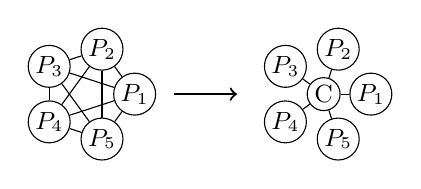
\begin{tikzpicture}[baseline, every node/.style={circle, draw, fill=white, inner sep=1pt, font=\small, minimum size=2mm}]
					\foreach \i in {1,...,5} {
						\node (n\i) at ({72*(\i-1)}:0.6) {$P_{\i}$};
					}
					\foreach \i in {1,...,5} {
						\foreach \j in {1,...,5} {
							\ifnum\i<\j
								\draw (n\i) -- (n\j);
							\fi
						}
					}

					\draw[->, thick] (1.1,0) -- (1.9,0);

					\begin{scope}[xshift=3cm]
						\node (c) at (0,0) {C};
						\foreach \i in {1,...,5} {
							\node (n\i) at ({72*(\i-1)}:0.6) {$P_{\i}$};
							\draw (c) -- (n\i);
						}
					\end{scope}
				\end{tikzpicture}
			\end{center}
			\pause
			\begin{block}{Netting}
				Centralisation allows for \textbf{netting} of rights and obligations. For any settlement time $T$, I only need to keep track of the difference between money owed to and by me, and units owed to and by me.
			\end{block}
		\end{column}

		\pause
		\begin{column}{0.48\textwidth}
			\begin{block}{Collateralisation}
				At certain intermediate times $t'$ ($t\leq t'\leq T$), participants may be required to physically give (`post') something to the exchange to \textbf{collateralise} their obligations.
				\begin{enumerate}
					\item Money (`margin') %Explain the term "futures type settlement" and "stock type settlement"
					\item Assets (`locate'/`borrow') %"Borrow" is only if you don't own the thing
				\end{enumerate}
				If an agreement made on the exchange gives you rights to money or assets, this is typically as good as posting actual money or assets.
			\end{block}
		\end{column}
	\end{columns}
\end{frame}

\begin{frame}{Summary}
	\begin{enumerate}
		\item \textbf{Trading} is swapping money and assets
		\item A \textbf{market} is whatever you use to trade
		\item A \textbf{securities market} is a standardised way to agree to trades
		\item Agreements consist of \textbf{rights} and \textbf{obligations}
		\item A \textbf{securities exchange} is a centralised trading venue %Maybe explain national market system
		\item After trades are agreed to, they will be \textbf{settled} in some standardised way
		\item Traders may be obligated to post assets ('locate') or money ('margin')
	\end{enumerate}
\end{frame}

\section{Trading}
\begin{frame}{Profitability}
	A sequence of trades that collectively increases the amount of money you have and leaves the amount of each asset you have unchanged is clearly favourable.

	Suppose that at each time $t$ you have cash holdings of $\$c_t$ and net holdings of $a_t$ units of some asset $A$.

	If you make trades $(s_t,q_t,p_t)$ at times $t \in \tau = \{t_0,\ldots, t_n\}$, then we will have
	$$a_{t_1} - a_{t_0} = \sum_{t\in \tau} s_t q_t$$
	%$$c_{t_1} - c_{t_0} = \sum_{t\in\tau} - p_t s_t q_t =  \int_{t\in\tau} -p_t da_t\footnote{$da_t$ is the Radon-Nikodym derivative of $a_t$ with respect to the counting measure of $\tau$.} \pause = p_{t_1}a_{t_1}-p_{t_0}a_{t_0}$$

	Suppose you make trades $(s_t,q_t,p_t)$ at times $t$. The change in your cash holdings $\Pi_t$ will be
	$\Pi = $
	The net change in our cash holdings as a result of a sequence of trades $ will be
	$$\Pi_{\mathcal{T}}=\sum_{\tau\in\mathcal{T}} -s_\tau q_\tau p_\tau.$$

	Consider the set of all our trades made in some time period $[0,T]$ for a particular asset. For any $t\in[0,T]$, our position $x_t$ will satisfy
	$$x_t - x_0 = \sum_{\tau : t_\tau \leq t} s_\tau q_\tau.$$
	Our cash holdings $\Pi_t$ will satisfy
	$$\Pi_t - \Pi_0 = \sum_{\tau : t_\tau \leq t} -p_\tau s_\tau q_\tau = \int_0^t p_t dx_t$$ %p_t is (our) LTP

	a db = [ab] - b da


	Consider a day's worth of trades for a single asset. I begin at time $0$ with a net position of $0$. My position at time $t$ is given by
	$$x_t = \int_0^t dx_t,$$
	where $\int_a^b dx_t$
	
	%Mark to market valuation
	%Portfolio value
	\begin{block}{Portfolio Capitalisation}
		Because of collateralisation requirements, \textbf{the amount you can trade (and therefore your potential profit) is constrained by how much money you have at the exchange.}
	\end{block}
	
	% Portfolio value integration by parts: pos dprice ~ price dpos
	% Dot products explainer
	% Portfolio returns and log-returns
\end{frame}

\begin{frame}{Trade Formation}
	On an electronic exchange, trade prices are determined by participants interacting with the exchange's \textbf{matching engine}.%Explain this term

	The most common type of matching engine is a \textbf{limit-order book}, which can operate in either a \textbf{continuous} or \textbf{batched} fashion.

	\pause
	
	\begin{block}{Limit-Order Book} %Special kind of data structure. Also called a double auction
		At any point in time, market participants can create a request (`\textbf{limit order}') to trade up to $q$ units at a price $p$ (or better). %Explain 'better'
		
		They are then said to be ``\textbf{bid} for $p$'' (if requesting to buy) or ``\textbf{ask}ing at $p$'' (if requesting to sell). %Bid and ask are terms referring to limit order directionality

		All limit orders are collected into a \textbf{limit-order book}. Orders may then be \textbf{cancelled}, \textbf{modified}, or \textbf{matched}. %matching is also called a fill

		%Limit orders are options provided to other market participants

		%Explain matching
		%Explain market orders as a bid for infty or an ask at 0

	\end{block}
	\begin{block}{Continuous Matching}
		% aggressive vs passive (taking/making)
		%adverse selection -> order priority. + free messages -> tick size, min size, lot size, ratelimits.
		% order priority -> latency -> colocation, fpgas.
	\end{block} %Usually used for intraday trading

	\begin{block}{Batch Matching}
		
	\end{block} %Usually used for opening and closing auctions ie day-open/day-close/lunchtime, or 
\end{frame}

\begin{frame}{Market Data \& Market Prices}
	In order to inform trading activity, market participants receive certain data about the orders and trades on the exchange.
	% Theoretical value
		% Efficiency
		% Liquidity
			% Decomposition of p&l into theo and execution
			% Market maker as liquidity provider

	% LTP
	% Price chart. Various position charts.
	% Microstructural noise -> Roll model

	% "lit" exchange just means more market data is made public

	% Order book diagram

\end{frame}

\begin{frame}{Valuation}
\end{frame}

\begin{frame}{Transaction Costs}
	% Fees
	% Spreads
	% Persistent price impact

	% Augmented P&L integral

	% Market impact
		% Adverse selection
		% Trade volumes and liquidity reinforce each other
\end{frame}

\begin{frame}{Uncertainty}
	%Dutch books & FTAP & Q vs P quant. Complete markets, arrow securities
	%(No-)Arbitrage (buy low sell high. Setup for statarb later)
\end{frame}

\begin{frame}{Decision-Making}
	%Systematic, semi-systematic, discretionary
	%High-touch, low-touch
	% What is point of systematic? (consistency, breadth)
		% “We’re mediocre traders, but our system never has rows with its girlfriends — that’s the kind of thing that causes patterns in markets.” Nick Patterson RenTech
\end{frame}

\section{Portfolio Management}
\begin{frame}{Risk}
	% Trading is zero-sum. So why do we do it
	% Risk = variance
		% "Cars have brakes so you can drive faster." Ben Rady
	% Portfolio variance and covariance
\end{frame}

\begin{frame}{Decision Theory}
	%Markowitz frontier
	%Pareto optimality
	%Security market line
	%Markowitz solution
		%Estimation difficulties
	%VNM & kelly theory
\end{frame}

\begin{frame}{Capital Asset Pricing Model}
	% Arbitrage arguments
	%Efficient Markets
	%Index investing. (Stats?)
		%Why ASX200 and not all ords (microstructure)
		%Grossman-Stiglitz Paradox
\end{frame}

\begin{frame}{Factor Models}
	% Mathematics
	% Sectors
	% Fama French
	% Factor models approximate cov matrix
		% Why cov matrix approximation is hard to begin with - paleologo 4.5.2 faq 4.5
	% Overrepresentation -> equal weighting (equal weighting index)
	% Factor loadings can't be centred (paleologo 4.4.1) unless an "equal weighting" vector is included
	% Types (paleologo 4.6):
		% characteristic
		% statistical
			% Latent factors (eg principal components)
		% macroeconomic
			% Fama macbeth
\end{frame}

\begin{frame}{Statistical Arbitrage}
	% Factor model stat arb (eg pairs trading), kalman filter with factor cov structure
\end{frame}

\section{Options Trading}
	%If black scholes was true options markets wouldnt exist

	% Linear regression mathematics
		% Matrix multiplication
	% Regularisation
	% Factor models in options pricing
		% Diagnosing issues with the model eg because black scholes is wrong ("all models are wrong")
\end{document}
